\newpage
\section{Cluttered Pick Test}

\subsection{Purpose and Focus of the Test}

The purpose of the \iaterm{Cluttered Pick Test}{CPT} is to evaluate the perception
and manipulation of the robots when objects are not seperated.

The scenario is motivated by the fact that most of the objects in the factory or 
labs are not perfectly placed but may be stacked or cluttered across a table.

Robots should be able to successfully grasp such objects in a way that they can place them somewhere else.
This ensures that they pick objects regarding potential further use.

\subsection{Scenario Environment}

The scenario is an alternated Basic Manipulation Test, with two service areas with a height of 10cm involved.
All available objects must be placed randomly in a box, which then is emptied above one table. The positions of the objects must remain as they fall. Objects that end up outside of the manipulation zone may be gathered, placed in the box and dropped again. The rule for a minimum distance of 0.02m between objects does not apply for this test. They may be placed near and on top of each other (see \ref{fig:clutter}).

\begin{figure} [h!]
\begin{center}
\subfloat[]{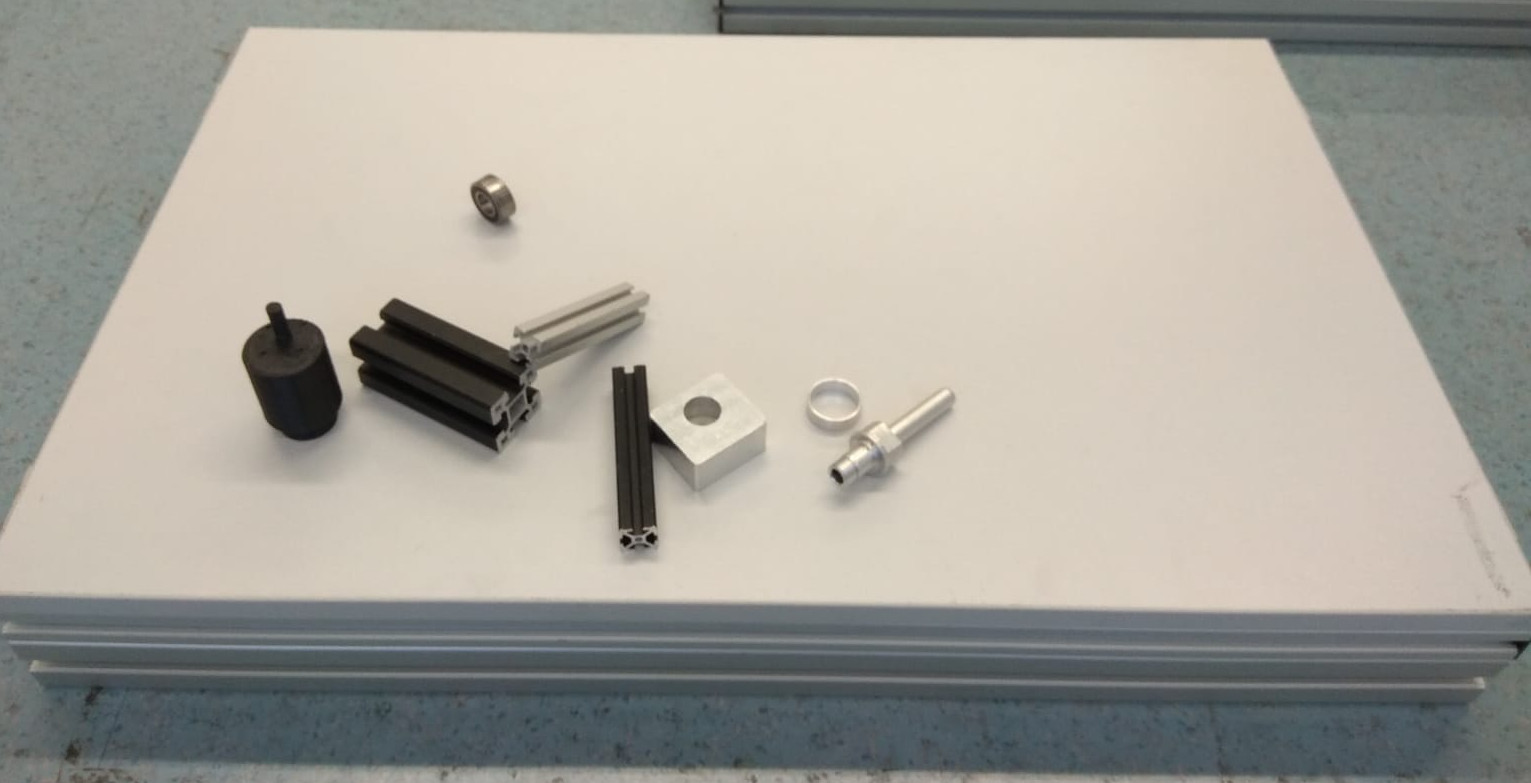
\includegraphics[height = 3cm]{./images/cluttered_pick_1.jpg}} \hspace{1cm}
%\subfloat[]{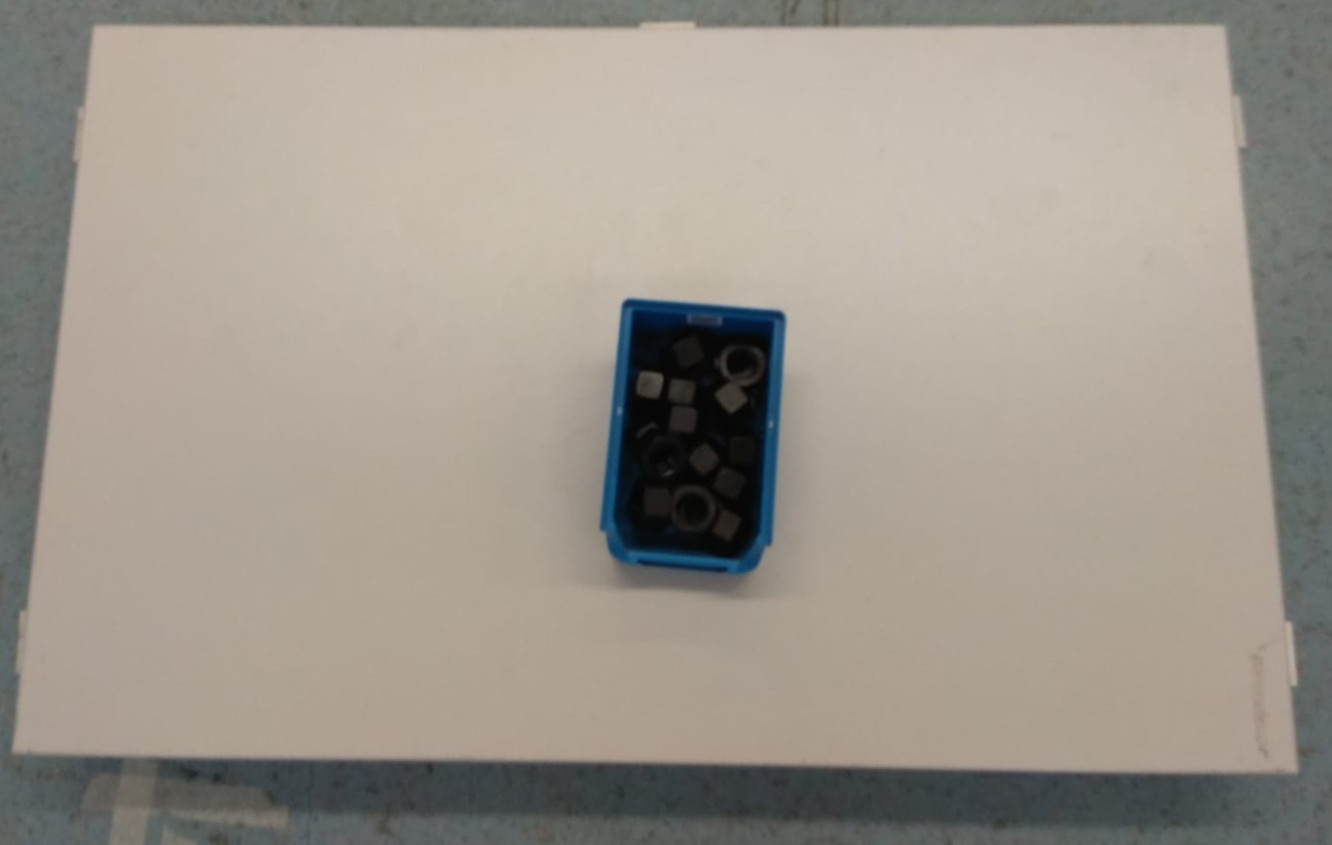
\includegraphics[height = 3cm]{./images/cluttered_pick_2.jpg}}
\end{center}
\caption{objects places in cluttered environment}
\label{fig:clutter}
\end{figure} 


%\subsection{Variation}
%A slight variation in the competition will be to run with 2 robots simultaneously competing with each other.
%For fairness of the competition the organizers should ensure that the distance between the robot starting
%point and the corresponding service station be equal.

\subsection{Task}

The task is the same as for a BMT, with the modification that only 3 objects must be picked and placed.

\subsection{Rules}
The following rules have to be obeyed:

\begin{itemize}
\item A single robot is used.
\item Three objects have to be picked.
\item There must be atleast 5 decoy objects which must not be picked.
\item The robot has to start from outside the arena and to stop in the goal area.
\item A manipulation object counts as successfully grasped as specified in Section~\ref{ssec:GraspingObjects}.
\item The run is over when the robot reached the final place or the designated time has expired.
\item The order in which the teams have to perform will be determined by a draw.
\item At the beginning of a team's period, the team will get the task specification.
\end{itemize}

\subsection{Scoring}
\begin{itemize}
\item 200 points are awarded for each correctly and successfully picked object
\item 125 points are awarded for each correctly placed object.
\item Standard scoring applies for all other aspects
\end{itemize}
